%!TeX root = ./../Bachelorarbeit.tex

%##########################################################
% Inhalt
%##########################################################

\clearpage
\chapter{Konzeption}

\section{Auswahl der Peripherie}
\label{sec:concept-periphery-selection}

Für diese Arbeit wurde das \textit{\ac{gpio}} und das
\textit{\ac{uart}}-Peripheriemodul für Tests und Implementierung ausgewählt.
Beide Schnittstellen sind für eingebettete Systeme unerlässlich und können für
verschiedenste Anwendungen eingesetzt werden.
\newline
UART wurde ausgewählt, da der Aufwand der Integration bereits in QEMU
bestehender Schnittstellen bewertet werden soll.
Es existiert bereits eine Implementation eines UART Controllers für einen
Mikrocontroller der STM32F2-Familie.
Da Mikrocontroller Modelle der STM32F2 und STM32F4 Familien Pin-kompatibel
sind, sollte die bestehende Implementation des UART Controllers ebenfalls
für den STM32F429 SoC verwendet werden können.
Darüber hinaus ist die Funktionalität von UART im Vergleich zu anderen
seriellen Schnittstellen einfacher zu testen.
Es können Funktionen wie ARM's \textit{Semihosting} verwendet werden, um
beispielsweise durch UART übertragene Zeichen in der Kommandozeile auszugeben.
Dies verringert die Komplexität der Testprogramme, da keine speziellen
Änderungen für die jeweilige Testumgebung (QEMU oder echte Hardware) erfordlich
sind.
\newline
Die GPIO Schnittstelle wurde für eine neue, eigenständige Implementierung in
QEMU ausgewählt.
Sie weist eine vergleichsweise geringe Komplexität auf.
Testprogramme für die GPIO Funktionalität sollten ebenfalls ohne Anpassungen
sowohl in QEMU, als auch auf echter Hardware laufen.
In QEMU Version 9.0 existiert bereits eine Integration für einen
Mikrocontroller der STM32L4-Familie.
Das GPIO-Peripheriemodul der STM32L4-Familie ist allerdings nicht kompatibel
zum GPIO-Peripheriemodul der STM32F4-Familie.
Es verfügt über eine andere Anzahl an Peripherie Registern, mit anderen
Funktionalitäten.
Die Implementierung kann daher nur als Orientierung dienen und muss
entsprechend angepasst werden.

% TODO: Entwicklungsumgebung
% TODO: Unterschied Simulation und Emulation
\section{QEMU Erweiterung}

QEMU unterscheidet bei der Emulation von ARM Systemen zwischen Maschinen und
\ac{cpu}'s.
Die Maschine ist in der Regel ein spezielles Entwicklungsboard eines
Herstellers, welches einen \ac{soc} auf einer Leiterplatte integriert, zum
Beispiel das STM32F429-Discovery\cite{Stm32F429DiscoveryBoard} oder das
Olimex-STM32-E407\cite{OlimexStm32E407Board}.
\newline
In QEMU werden Maschine und SoC meist getrennt implementiert.
Die Maschine, bzw. das Entwicklungsboard, agiert dabei als Container für den
SoC.
Die meisten Funktionalitäten, sowie die Peripherie, werden im SoC
implementiert und der Maschine zur Verfügung gestellt.
Die CPU ist für die meisten \acp{soc} festgesetzt, da auf der echten Hardware
ebenfalls standardmäßig nur eine CPU zur Anwendung kommt.
Die CPU Architektur des STM32F429 Mikrocontrollers, \textit{Cortex-M4F} kann
vollständig in QEMU emuliert werden.
Beide der folgenden Ansätze sollen die CPU Emulation nutzen und um bestimmte
Peripherien erweitern.

% TODO: EXTI benutzen?
\subsection{QEMU Device Implementierung} \label{konzept-qemu-dev}

Zunächst soll untersucht werden, wie eine Maschine und der dazugehörige SoC
direkt in QEMU integriert werden kann.
Das QEMU Projekt ist bereits über 20 Jahre alt und verfügt über diverse
\acp{api}.
Diese sollen genutzt werden um das Projekt durch den STM32F429-\ac{soc} zu
erweitern.
Desweiteren soll eine Maschine integriert werden welche den \ac{soc}
implementiert.
Der grobe Ablauf dieser Erweiterung besteht also aus folgenden Abschnitten:
\begin{enumerate}
    \item Hinzufügen neuer Build-System Konfiguration für \ac{soc},
    \item Implementierung des STM32F429-\ac{soc},
    % TODO: Spezifiziere welche Peripherie
    \item Integration bestehender Peripherie in \ac{soc},
    \item Hinzufügen neuer Build-System Konfiguration für GPIO-Peripherie
    \item Implementierung der neuen Peripherie und Integration in \ac{soc}
\end{enumerate}
Die Adressen der Peripherie müssen dem Technischen-Referenzwerk des
STM32F429-Mikrocontrollers entnommen werden.
Die Funktionsweise und Konfiguration der Peripherie-Register sind dort
ebenfalls beschrieben.
\begin{figure}[!htb]
    \centering
    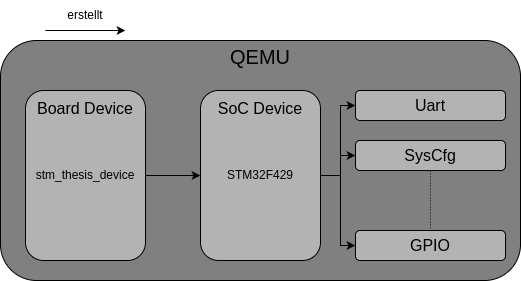
\includegraphics[width=0.7\textwidth]{anlagen/bilder/Qemu_Device}
    \caption{Grobe Skizzierung der Interaktion zwischen Maschine, \ac{soc} und Peripherie}
    \label{fig:QemuDeviceErweiterung}
\end{figure}


% TODO: Kompilieren von EDI Repo mit libnanomsg
\subsection{External Device Interface Implementierung}

Im zweiten Ansatz soll ein weiteres Konzept für die Integration neuer
\ac{soc}'s in QEMU vorgestellt werden.
Bei dieser Methode wird die Implementierung der Peripherie in externe Prozesse
verlagert.
Die Unterscheidung zwischen CPU und Maschine besteht zwar auch bei diesem
Ansatz, allerdings ist der Funktionsumfang der Maschine stark reduziert, da sie
keine Peripherie direkt über den \ac{soc} integriert.
Die relevanten Schnittstellen laufen jeweils gekapselt in einem separaten
Prozess und kommunizieren mittels \ac{ipc} mit der QEMU-Anwendung.
\begin{figure}[!htb]
    \centering
    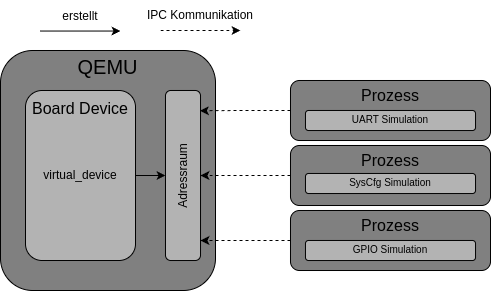
\includegraphics[width=0.7\textwidth]{anlagen/bilder/Qemu_external_device}
    \caption{Grobe Skizzierung der Interaktion zwischen QEMU und externen Prozessen}
    \label{fig:QemuExternalDeviceErweiterung}
\end{figure}
Dies ermöglicht eine unabhängige Implementierung von Peripherie und \ac{soc}.
Die Interprozesskommunikation wird mittels einer externen Bibliothek
realisiert, welche in die QEMU Anwendung integriert werden muss.
Im Gegensatz zum ersten Ansatz muss nicht für jeden neuen Mikrocontroller eine
separate Maschine mitsamt \ac{cpu} implementiert werden.
Stattdessen reicht eine generische Maschine welche den jeweiligen \ac{cpu}-Typ
integriert.
Um die Komplexität gering zu halten soll nur die im STM32F429-\ac{soc}
verwendete \ac{cpu} benutzt werden.
Die Verbindung von QEMU-Emulation und den separaten Prozessen erfolgt bei Start
der QEMU-Anwendung.
Dort können einzelne Devices oder eine Gruppe von Devices mit einer
spezifischen Adresse im Adressraum des \ac{soc} verbunden werden.

% TODO: Was sind Voraussetzungen für Programm?? -> zusätzlich zu Startup auch Tick und anderes
% TODO: Wieso kein StmCube und/oder Keil MDK ARM
% TODO: Wieso meson, wie funktioniert meson mit cross compile
% TODO: Wie sind Testaufbauten geplant? -> Richtige Testaufbauten dann in Implementaiton
% TODO: Projektaufbau
% TODO: Vergleichende tests qemu und hardware
% TODO: Bei gpio test Programm -> Falls timer nicht abstrahiert einfach loop zählen lassen
\section{Testprogramme und Teststrategie}

Um die korrekte Funktionsweise der Peripherie und \ac{soc} Implementierungen zu
testen sollen verschiedene Testprogramme entwickelt werden.
Diese Testprogramme werden anschließend sowohl in QEMU als auch auf realer
Hardware ausgeführt.
Da bei allen Ansätzen der gleiche \ac{soc} mit gleicher \ac{cpu} eingesetzt
wird reicht es die Tests auf die jeweilige Peripherie zu beschränken.
Während der Ausführung können unterschiedliche Verhalten in der Software für
emulierte und reale Umgebung auftreten.
Um diese möglichst gering zu halten sollen die Testprogramme eine möglichst
geringe Komplexität aufweisen.
\newline
Für die Entwicklung der Tests sollen ausschließlich die notwendigsten externen
Bibliotheken genutzt und konfiguriert werden.
Dies umfasst die STM-\textit{\ac{hal}}, für Programmierung und Konfiguration
der Peripherie.
Zur Konfiguration der der \ac{cpu} spezifischen
Einstellungen soll das \textit{\ac{cmsis}} verwendet werden.
Die eigentliche Testanwendung wird dann in \textit{C} programmiert.
Für die Testprojekte wird das Build-System \textit{Meson} verwendet, da dies
auch im QEMU Projekt zum Einsatz kommt und somit keine erneute Umgewöhnung
erfordert.
